\documentclass[12pt,titlepage]{article}

\usepackage{ngerman,amsmath,graphicx,a4wide,fontspec,hyperref}
\setmainfont{Helvetica Neue}
\setmonofont{Menlo Regular}

\begin{document}

\title{Miniprojekt: \\ Minimax-Maschine \\ Dokumentation}
\author{Clemens Pollak, Robin Thrift, Max Boll}
\date{Hardware Projekt 2014 \\ 11.11.2014}
\maketitle

\tableofcontents

\newpage

\section{Einleitung} 
Unser gew{\"a}hltes Thema befasst sich mit der Minimax-Maschine und mit der Realisierung von Algorithmen auf ihr. Dieses Thema soll im Rahmen des Hardware Praktikums bearbeitet werden und ist uns aus der Veranstaltung "'Grundlagen der Rechnerarchitektur"' bereits grundlegend bekannt.\\ Um unsere Vorbereitung auf dieses Projekt dokumentieren und strukturieren zu k{\"o}nnen, erstellen wir ein Pflichtenheft. Dieses Pflichtenheft wird nur unsere Vorbereitung beinhalten und es wird au{\ss}erdem eine weitere Dokumentation der Ergebnissen geben. Außerdem wird es w{\"a}hrend der Bearbeitung unseres Projects einen Leitfaden für uns darstellen, der die Implementierung der L{\"o}sung vereinfacht und beschleunigt.


\section{Aufgabenstellung}
Nach unserem Verst{\"a}ndniss ist das Ziel dieser Aufgabenstellung ein Algorithmus, welcher auf der Minimax-Maschine zu implementieren ist und eine sogenannte Paketanalyse betreibt. Dieser "'Paketanalyse"'-Algorithmus befasst sich mit dem Datenpaketen, welche im Speicher der Minimax-Maschine abgelegt sind.\\ Ein Datenpaket beginnt immer mit der Folge "'1110"' und besteht aus einem
Kopf mit einer L{\"a}nge von 80 Bits und einem Datenteil mit variabler L{\"a}nge. Der Kopf enth{\"a}lt die Kanalnummer zwischen der 32. und 47. Bitstelle. Zu einem Kanal k{\"o}nnen ein oder mehrere Pakete geh{\"o}ren, welche die selbe Kanalnummer haben.
Die Anzahl Bits, welche in den Speicher geladen werden, welche überprüft werden müssen wird als bekannt vorausgesetzt und wird in ein entsprechendes Register vorgeladen.\\
Nun soll der Algorithmus eine Datentabelle anlegen, welche sich au{\ss}erhalb der Speicherfelder der einzelnen Pakete befindet. Diese Datentabelle soll den Kanalnummern die L{\"a}ngen der jeweiligen Datenteile aller Pakete zuordenen um dann später exportiert zu werden. Diese Aufgabenstellung soll mit dem Minimax-Simulator simuliert und getestet werden. Die Maschine kann durch vorgegebene Bauteile erweitert werden, was sich aber auf die Bewertung auswirkt. Der Algorithmus wird in Form der sogenannten Steuertabelle implementiert und soll außerdem als Flussdiagramm abgegeben werden.

\newpage

\section{Ist-Analyse der Basis-Maschine}

Die Minimax-Maschine ist ein minimales Rechensystem welches aus einfachen Registern (Basis: \texttt{ACCU}, \texttt{PC}, \texttt{IR}, \texttt{MDR}, \texttt{MAR};
weitere k{\"o}nnen hinzuge{\"u}fgt werden), einer arithmetisch-logischen Einheit (ALU) und einem Hauptspeicher (HS) aufgebaut
ist und durch ein Mikropgramm gesteuert wird. Jedes dieser Register hat als Eingang mindestens die ALU und hat zusätzlich einen Eingang, der den Schreibzugriff regelt.\\
\begin{enumerate}
\item \texttt{ACCU}: Abk{\"u}rzung f{\"u}r "'Accumulator"' ein Zwischenspeicher, um mit \texttt{MDR} Operationen durchführen zu k{\"o}nnen.
\item \texttt{PC}: Abk{\"u}rzung f{\"u}r "'program counter"', enthält den Programmzähler, welcher den nächsten Befehl beeinflusst
\item \texttt{IR}: Abk{\"u}rzung f{\"u}r "'instruction register"', enthält Opcode(8 Bit) und Adressteil(24 bit).
\item \texttt{MDR}: Abk{\"u}rzung f{\"u}r "'memory data register"', enthält je nach Einstellung des Multiplexers texttt{MDR.Sel}, verschiede Daten entweder aus Hauptspecher oder aus der \texttt{ALU}.
\item \texttt{MAR}: Abk{\"u}rzung f{\"u}r "'memory adress register"', enth{\"a}lt die Speicheradresse an der aus dem Hauptspeicher Daten geladen oder geschrieben werde sollen.
\item \texttt{HS}: Abk{\"u}rzung f{\"u}r "'Hauptspeicher"', er wird mit 24-Bit durch \texttt{MAR} adressiert und gibt eine 32-Bit Zahl zur{\"u}ck. Auf die selbe Art funktioniert schreiben einer 32-Bit Zahl nat{\"u}rlich auch.
\end{enumerate}

\leavevmode \\

\begin{enumerate}
\item \texttt{ADD}: Addiert ALU-Eingang A und ALU-Eingang B
\item \texttt{SUB.B}: Subtrahiert ALU-Eingang A von ALU-Eingang B
\item \texttt{TRANS.A}: Schaltet den ALU-Eingang A durch
\item \texttt{TRANS.B}: Schaltet den ALU-Eingang B durch
\end{enumerate}

\leavevmode \\

Dabei sind die m{\"o}glichen Operationen auf die in der ALU implementieren
Operationen beschr{\"a}nkt (Basis: \texttt{ADD}, \texttt{SUB.B}, \texttt{TRANS.A}, \texttt{TRANS.B}). Die ALU kannn mit weiteren Operationen,
wie z. B. dem bitweisen UND, erg{\"a}nzt werden.\\
Um eine Operation auszuf{\"u}hren m{\"u}ssen {\"u}ber die Multiplexer \texttt{ALUSel.A} und \texttt{AluSel.B} zwei Operanden ausgew{\"a}hlt werden
und der ALU muss {\"u}ber die \texttt{ALU Ctrl}-Leitung der Code f{\"u}r die Operation {\"u}bergben werden. An den Multiplexern liegen sowohl
Konstanten als auch die Register an, welche zur ALU durchgeschaltet werden k{\"o}nnen. Das Ergebnis der Operation kann
entweder in einem Register oder (über MDR) im HS (Adresse im Register \texttt{MAR}) gespeichert werden. Zus{\"a}tzlich k{\"o}nnen s. g. Flags (Basis nur ein Flag \texttt{ALU RESULT == 0})
gesetzt werden, welche zur{\"u}ck zur Control Unit (CU) geleitet werden um z. B. bedingte Spr{\"u}nge auszuf{\"u}hren.

Abbildung 1 zeigt die uns vorliegende Basismaschine.

\leavevmode \\

Die uns vorliegende Minimax-Maschine arbeitet mit 32-Bit und speichert Werte mit 32-Bit in den Registern und im HS (\dq Little Endian\dq ).
Alle ALU-Operationen werden folglich alle mit 32-Bit ausgef{\"u}hrt. Dies stellt sich jedoch f{\"u}r unser Aufgabe als
Hindernis, da wir die Daten bitweise untersuchen m{\"u}ssen, Daten aus dem HS und den Registern jedoch nur als
32-Bit Zahlen auslesen k{\"o}nnen und nicht als einzelne Bits.

Folglich wird die Basismaschine um einige Konstanten, Operationen und Register erweitert werden müssen, welche im "'Implementierungskonzept'" n{\"a}her
aufgeführt sind.

\newpage

\section{Finale Implementierung}
Wir haben das Hauptproblem in einige Teilprobleme aufgeteilt:
\begin{enumerate}
\item Das sequenzielle Auslesen des Hauptspeichers
\item Die Analyse der Daten
    \begin{enumerate}
    \item Das erkennen der Startsequenz eines neuen Pakets
    \item Das Auslesen der Kanalnummer
    \end{enumerate}
\item Das speichern der geforderten Daten im HS
\end{enumerate}

\subsection{Sequenzielles Auslesen aus dem Hauptspeicher}
Zun{\"a}chst m{\"u}ssen also die abgelegten Daten sequenziell ausgelsen werden. Da die Anzahl der in den Speicher geladenen Bits
bekannt ist (im Register \texttt{LNGTH} abgelegt), kann hierzu ein Mirkoprogramm implementiert werden, welches mithilfe
einer Schleife alle Speicherzellen ausliest, bis die Anzahl der ausgelesenen Bits gleich der Zahl im Register \texttt{LGNTH} ist.
Hierzu muss die Minimax-Maschine um ein Register erweitert werden, welches die akutelle Speicheradresse enth{\"a}lt (anfangs 0),
und mit wir \texttt{ADDR} bezeichnen werden. Bei jeder Iteration wird der Wert an der Adresse \texttt{ADDR} im Register 
\texttt{MDR} gespeichert und steht somit dem Analyseprogramm zur Verf{\"u}gung. Nach der Analyse wird das Register \texttt{ADDR}
inkrementiert und es wird zur{\"u}ck zum Schleifenkopf gesprungen (Siehe Abb. 1 im Anhang).

\subsection{Analyse der Daten}
Die Analyse der Daten kann als einfacher endlicher Automat mit 2 Zuständen betrachtet werden (0, 1). Im ersten Zustand (0)
wurde noch kein Paket gefunden und es wird mit Hilfe einer Bitmaske ($1111_{2} = 15_{10}$) nach der Anfangssequenz gesucht. 
Wenn die Startsequenz gefunden wurde wird der Zustand verändert (zu 1) und es wird auf die nächste Zahl aus dem HS gewartet. 
In der nächsten Zahl aus dem HS befindet sich die Kanalnummer. Diese wird mit einer weiteren Bitmaske ausgelesen
und im Register \texttt{CHNL} abgelegt.
Wurde sowohl ein Packetanfang als auch eine Kanalnummer gefunden, so wird nun die Länge des Datenfeldes gezählt und im Register \texttt{DATAC} gespeichert, bis erneut die Startsequenz gefunden wird.
Wurde eine neue Startsequenz gefunden so wird von der Länge des Daten 16 abgezogen (16 Bits Overhead des Headers) und
es wird an das Speicherprogramm angegeben und es wird wieder in den zweiten Zustand (1) gewechselt.

\subsection{Ablegen der Daten im Hauptspeicher}
Ziel der Analyse ist es die Länge aller Datenpakete für jeden Kanal zu z{\"a}hlen und in eine Tabelle im Hauptspeicher abzulegen.
Dazu wird zunächst eine Anfangsadresse (Offset) gewählt (Register \texttt{OFFSET}), welche unsere Tabelle weit von den Eingabedaten
im Hauptspeicher plaziert. Die Tabelle wird als einfaches indiziertes Array modelliert, in welchem die Kanalnummern die
Schlüssel sind. Nach dem Auslesen der Kanalnummer (abgelegt im Register \texttt{CHNL}) wird also die Speicherzelle mit der Adresse 
$\texttt{ACCU} + \texttt{OFFSET}$ mit Datenlänge (Register \texttt{DATAC}) addiert und an der gleichen Stelle wieder abgelegt (Siehe
Abb. 3 im Anhang)

\section{Angestrebte Projektergebnisse}
\begin{enumerate}
\item Die Tabelle, in der die einzelnen Kanalnummern und Paketl{\"a}ngen enthalten sind. (Als exportierte Speicherdatei)
\item Eine Dokumentation, welche unserer Implementierung im Detail beschreibt und m{\"o}glicherweise schwierige Stellen verst{\"a}ndlich erl{\"a}utert.
\item Einen exportierten Schaltplan der erweiterten Minimax-Maschine.
\end{enumerate}

\section{Projektdurchf{\"u}hrung}

\subsection{Zeitlicher Ablauf der Projektarbeit}

\begin{itemize}
\item [] \textbf{20.10.14} Besprechung des unseres Hardware Projekts
\item [] \textbf{31.10.14} Abgabe Pflichetenheft mit grober Skizze der L{\"o}sung
\item [] \textbf{05.11.14} Besprechung des Pflichtenhefts und Anfang der Implementierung des Problems
\item [] \textbf{14.11.14} Geplante Abgabe der Dokumentation des Projekts
\item [] \textbf{20.11.14} Geplante Pr{\"a}sentation unserer Lösung
\end{itemize}

\subsection{Erweiterungen der Minimax-Basis-Maschine}

\subsubsection{Register}

\begin{enumerate}
\item \texttt{COUNT}: Gesammtl{\"a}nge der Auszuwertenden Daten
\item \texttt{OFFSET}: F{\"u}r den Offsetwert, der bei der Speicherung der Längen addiert wird
\item \texttt{ADDR}: Ein Register f{\"u}r die aktuelle Adresse
\item \texttt{OLD}: Zwischenspeicher
\item \texttt{CHNL}: Hält die aktuelle Kanalnummer
\item \texttt{DATAC}: Zähler für Länge des Datenfeldes
\item \texttt{STATE}: Variable zum Speicher des States des Analyseautomaten
\end{enumerate}

\subsubsection{ALU-Opertationen}

\begin{enumerate}
\item placeholder
\end{enumerate}

\subsubsection{Konstanten}
Wir haben nur eine Konstante verwendet, diejenige die in dem Register \texttt{OFFSET} gespeichert ist. Sie beträgt: <value>

\subsubsection{Multiplexer-Eingänge}

ALUSel.A:

\begin{table}
    \begin{tabular}{l|l}
    Adresse & Wert              \\
    \hline  					\\
    000     & 0                 \\
    001     & 1                 \\
    010     & ACCU (Register)   \\
    011     & OFFSET (Register) \\
    100     & LNGTH             \\
    \end{tabular}
\end{table}

ALUSel.B:

\begin{table}
    \begin{tabular}{l|l}
    Adresse & Wert            \\
    \hline                    \\
    000     & MDR (Register)  \\
    001     & AT (Register)   \\
    010     & PC (Register)   \\
    011     & ACCU (Register) \\
    100     & OLD (Register)  \\
    \end{tabular}
\end{table}


\section{Anhang}

\subsection{Abb. 1: Basismaschine}
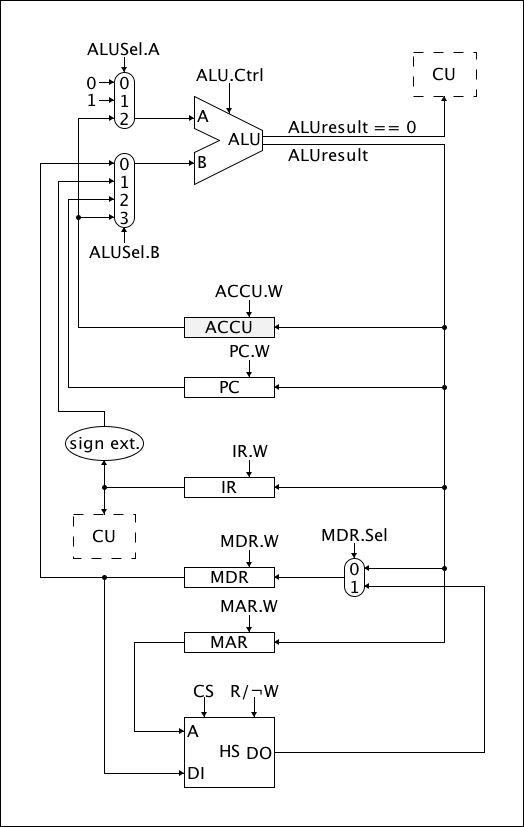
\includegraphics[width=13cm]{schematics.png}

\subsection{Abb. 2: Flussdiagramm des Speicherauslesepgrogramms}
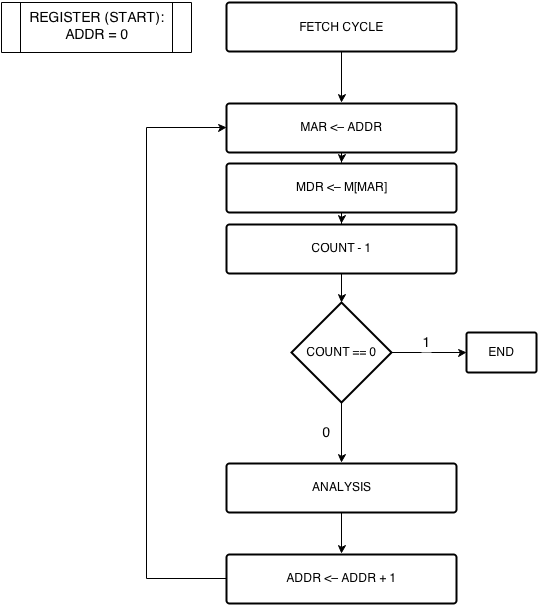
\includegraphics[width=13cm]{readFromMemory.png}

\subsection{Abb. 3: Flussdiagramm des Analyseprogramms}
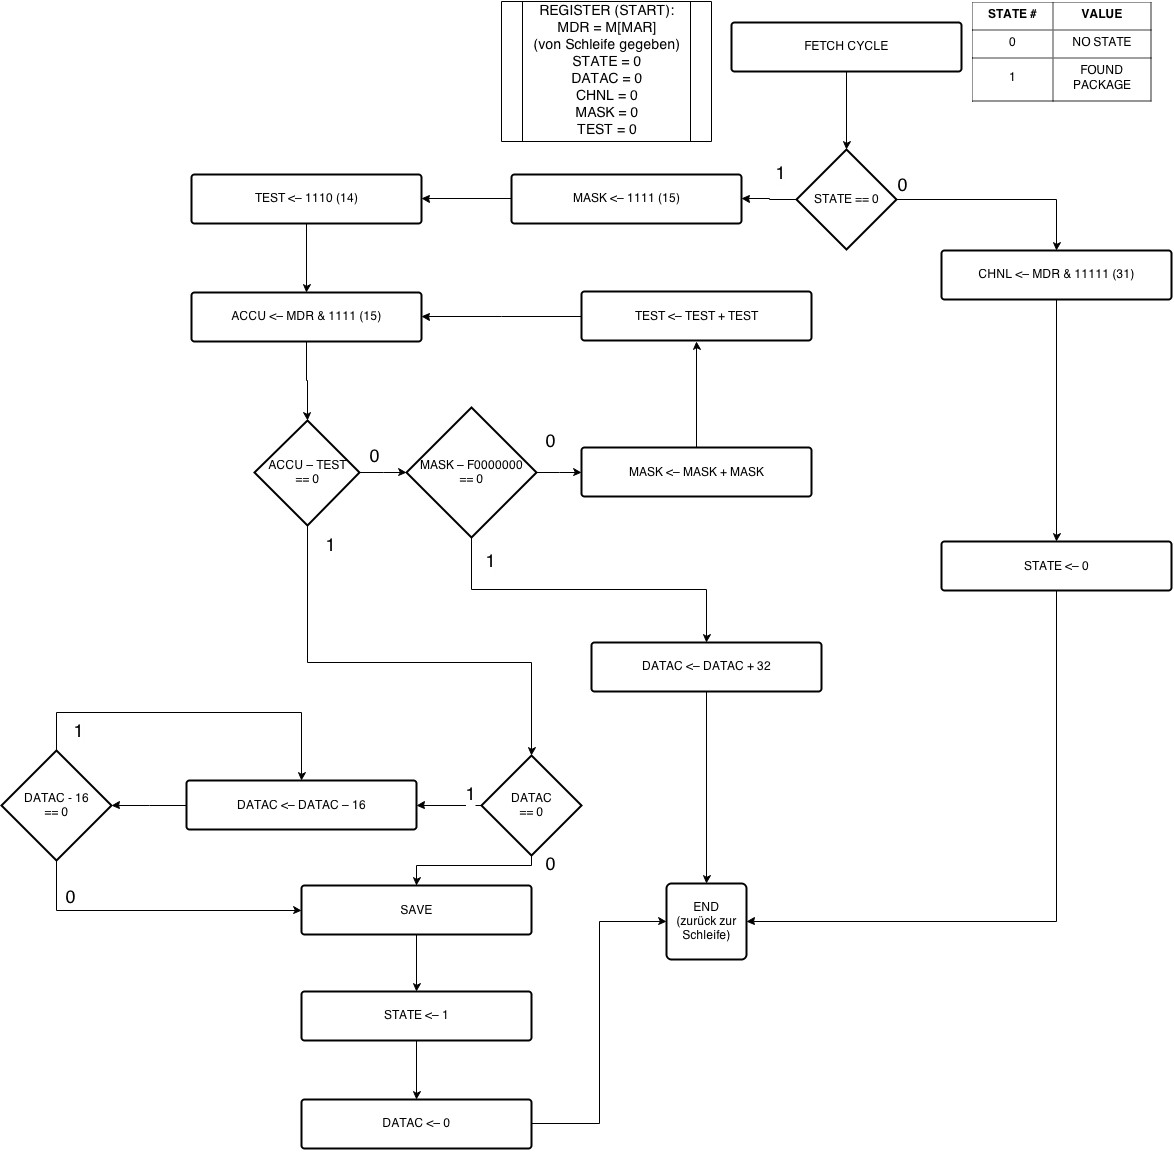
\includegraphics[width=13cm]{analyseData.png}

\subsection{Abb. 4: Flussdiagramm des Speicherprogramms}
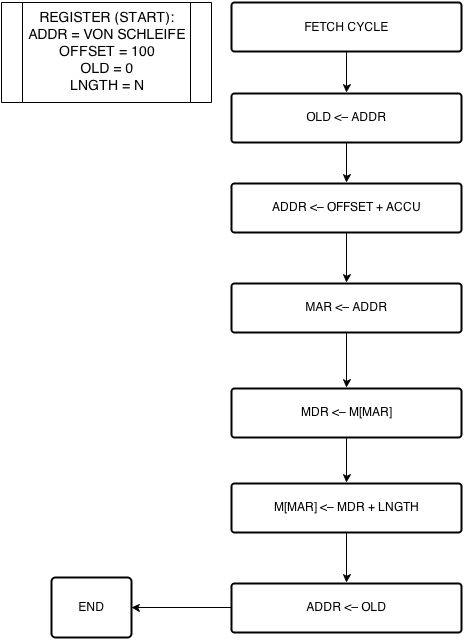
\includegraphics[width=13cm]{saveToHS.png}

\subsection{Abb. 5: Flussdiagramm des Programms zum Überspringen des Datenfeldes}
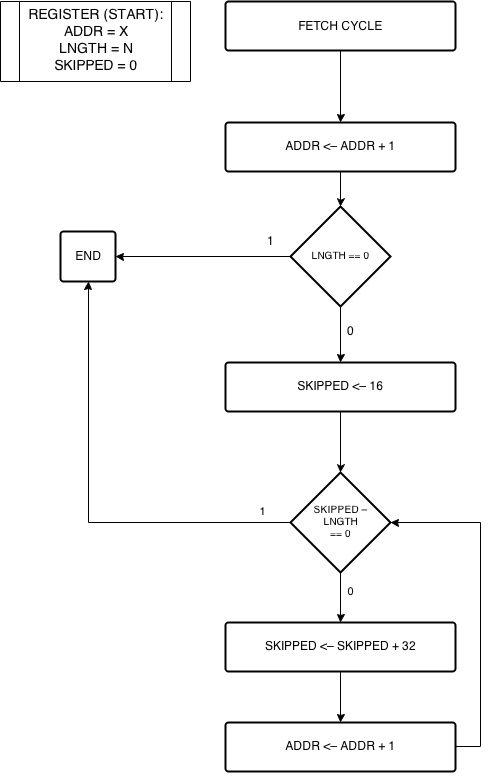
\includegraphics[width=10cm]{skipBits.png}

\newpage

\section{Arbeitsaufteilung}
Da sich das vorliegende Problem sehr gut in kleinere Teilprobleme aufteilen lässt ergibt sich folgende 
Arbeitsteilung:
\leavevmode \\
\\
\begin{tabular}{|l|c|}
\hline
Robin Thrift &  Analyse-Algorithmus der ausgelesenen Daten \\
\hline
Clemens Pollak & und sequentieller Einlesealgorithmus \\
\hline
Max Boll & Speicheralgorithmus \\
\hline
\end{tabular}
\leavevmode \\
\\
Dies beinhaltet auch die Dokumentation der jeweiligen Aufgabe (Da Git und LaTeX verwendet werden kann jedes 
Teammitglied gefahrenlos zur Dokumentation beitragen).


\section{Hilfsmittel}
Wir haben folgende Quellen benutzt:
\begin{enumerate} 
\item Wikipedia: \dq Mask (computing)\dq \\ \string[\url{http://en.wikipedia.org/wiki/Mask_(computing)}\string]
\item Wikipedia: \dq Bitweiser Operator\dq \\ \string[\url{http://de.wikipedia.org/wiki/Bitweiser_Operator}\string]
\item Git VCS zur Quellcodeorganisation und Synchronisation
\item GitHub zur Projektorgansation und Quellcodesynchronisation
\item Flowcharts: \string[\url{https://www.draw.io}]
\item SRA Minimax-Simulator
\item Informationsfolien (Aufgabenstellung)
\item Materialen der Veranstaltung \dq Grundlagen der Rechnerarchitektur\dq von Prof. Dr.-Ing. habil. Jürgen Brehm
\end{enumerate}

\end{document}
